\section{Representative Examples}

Given the theoretical framework for downfolding a many-orbital (or many electron) problem to a 
few orbital (or few electron) problem, we now discuss examples which elucidate the 
AIDMD method. 
%The first example is mostly pedagogical, 
%where we have completely avoided the \textit{ab-initio} related complications of AIDMD. Rather, we use information directly available 
%from \textit{exact} eigenstates themselves to downfold from a lattice model with more orbitals (3-band model) 
%to one with fewer orbitals (1-band model). We then gradually increase the complexity of the problems we address 
%by downfolding the hydrogen chain in one dimension (with up to 10 atoms) and graphene 
%(with up to 32 carbons on a 2D honeycomb lattice). Finally, we use the matching pursuit algorithm discussed 
%in section 2, suited for multiple energy scales, for the case of transition metals 
%by considering the diatomic FeSe molecule.
%\lucas{What about this? } \HJC{Yes, this is good} 
The examples are as follows:
\begin{itemize}
\item Section~\ref{subsection:3band}: Three band Hubbard $\rightarrow$ one band Hubbard at half filling. Demonstrates finding a basis set for the second quantized operators and uses a set of eigenstates directly sampled from the low-energy space to find a one-band model.
\item Section~\ref{subsection:1dhydrogen}: Hydrogen chain $\rightarrow$ one band Hubbard model at half filling. Demonstrates basis sets for {\it ab-initio} systems and the possibility to use this technique to determine the quality of a model to a given physical situation.
\item Section~\ref{subsection:graphene}: Graphene $\rightarrow$ one band Hubbard model with and without $\sigma$ electrons. Demonstrates using the downfolding procedure to examine the effects of screening due to core electrons. 
\item Section~\ref{subsection:fese}: FeSe molecule $\rightarrow$ $d,p,4s$ system. Demonstrates the use of matching pursuit to assess the importance of terms in an effective model and to select compact effective models.
\end{itemize}

\HJC{Lucas, Is this better?} \lucas{It still looks to me that this really goes in the 3-band part?} 
\HJC{1-band comes in several subsections, hence the need to define it early?}
In all examples we will highlight the important ingredients associated with AIDMD. First and foremost, is the choice 
of low energy space or energy window i.e. how our database of wavefunctions was generated. Associated with this is 
the choice of the one body space in terms of which the effective Hamiltonian is expressed. Finally, we discuss 
aspects of the functional forms or parameterizations that are expected to describe our physical 
problem. In three out of our four representative examples we work with the single (or 1-) band Hubbard Hamiltonian,
\begin{equation}
	\tilde{H} = -t \;\sum_{\langle i,j \rangle} \tilde{d}_i^{\dagger} \tilde{d}_j + U \;\sum_{i} \tilde{n}^{i}_{\uparrow} \tilde{n}^{i}_{\downarrow}
\label{eq:oneband}
\end{equation}
where $t$ and $U$ correspond to downfolded (renormalized) parameters and $\tilde{d}$ are the effective one-particle operators, 
which are obtained from transformations on their bare counterparts. 
%Thus 
%the determination of effective Hamiltonians is a \emph{dual} problem - what are the composite objects ($\tilde{d}_i$ here) 
%that give a compact description of the low energy physics? and given this choice what 
%are the effective interactions between them?

\subsection{Three-band Hubbard model to one band Hubbard model at half filling}
\label{subsection:3band} 
\HJC{Still editing - need to incorporate Lucas suggestions and new results for 8 site FCI}
Our first example is motivated by the high $T_c$ superconducting cuprates~\cite{Bednorz1986} that 
have parent Mott insulators with rich phase diagrams on electron or hole doping~\cite{Dagotto_RevModPhys, LeeWen_RevModPhys}. 
Many works have been devoted to their model Hamiltonians and corresponding parameter 
values~\cite{Emery, ZhangRice, tJSpalek, Hybertsen_PRB1989, Hybertsen_PRB1990, Pavirini, Kent_Hubbard}. 
The emergent consensus of the minimal model involving the oxygens is the 3-orbital or 3-band Hubbard model, 
\begin{eqnarray}
H &=&    \epsilon_p \sum_{j,\sigma} n^{p}_{j,\sigma} + \epsilon_{d} \sum_{i,\sigma}  n^{d}_{i,\sigma} 
	+ t_{pd} \sum_{\langle i,j \rangle, \sigma} \text{sgn}(p_i,d_j) \Big( d_{i,\sigma}^{\dagger} p_{j,\sigma} + \text{h.c.} \Big) \nonumber \\
  & &   + U_p \sum_{j} n^{p}_{j,\uparrow} n^{p}_{j,\downarrow} + U_d \sum_{i} n^{d}_{i,\uparrow} n^{d}_{i,\downarrow} + V_{pd} \sum_{\langle i,j \rangle} n^{j}_p n^{i}_d 
\end{eqnarray}
%\begin{eqnarray}
%H &=&    \epsilon_p \sum_{j,\sigma} n^{p}_{j,\sigma} + \epsilon_{d} \sum_{i,\sigma}  n^{d}_{i,\sigma} 
%	+ t_{pd} \sum_{\langle i,j \rangle, \sigma} \text{sgn}(p_i,d_j) \Big( d_{i,\sigma}^{\dagger} p_{j,\sigma} + \text{h.c.} \Big) + U_p \sum_{j} n^{p}_{j,\uparrow} n^{p}_{j,\downarrow} + U_d \sum_{i} n^{d}_{i,\uparrow} n^{d}_{i,\downarrow} + V_{pd} \sum_{\langle i,j \rangle} n^{j}_p n^{i}_d 
%\end{eqnarray}
where $d_i,p_j$ refer to the  $d_{x^2 - y^2}$ orbitals of copper (at site $i$) and $p_x$ or $p_y$ 
oxygen (at site $j$)  respectively and the signs of the hopping $t_{pd}$ between them are shown in Fig.~\ref{fig:threeband}. 
$\epsilon_d$,$\epsilon_p$ refer to the orbital energies, 
$U_d$, $U_p$ refer to strength of onsite Hubbard interactions and $V_{pd}$ refers to the 
strength of the density-density interactions between a neighboring $p$ and $d$ orbital. 
We keep the exposition simple and consider only the case where $\epsilon_p$, $t_{pd}$ (chosen to be $1.3$ eV throughout) 
and $U_{d}$ are non zero. Since we work with fixed number of particles we set $\epsilon_d = 0$, thus the 
charge transfer energy $\Delta \equiv \epsilon_p - \epsilon_d$ equals $\epsilon_p$ in our notation. 
We work in the hole notation; half filling corresponds to 2$\uparrow$ and 2$\downarrow$ holes on the $2\times2$ cell.
\begin{figure}[htpb]
\centering

\includegraphics[width=0.8\linewidth]{./Figures/three_band_figure.eps}
\caption{Schematic for downfolding the three band Hubbard model to the one band Hubbard model. 
The oxygen orbitals are completely eliminated to give "dressed" $d$-like orbitals of the one band model, with modified hopping 
and interaction parameters.}
\label{fig:threeband} 
\end{figure}	

It is our objective to determine what 1-band Hubbard model "best" describe the 3-band data, the former defined 
in terms of effective \textit{d-like} orbitals, $\tilde{d}$, which are mixtures of copper and oxygen orbitals; 
this optimal transformation also remains an unknown. This is a \emph{dual} problem - what are the composite objects 
($\tilde{d}_i$ here) that give a compact description of the low energy physics? and given this choice what 
are the effective interactions between them?

In addition, the "best" effective Hamiltonian description depends on the energy scale of interest. 
We first focus on the lowest scales and use our knowledge of the exact 
eigenstates of the 3-band and 1-band models to perform a state by state comparison. 
This is verified by the standard protocol (of section 2) in this energy window. Then, to build faith 
in the results, the predictions of the 1-band Hubbard parameters are tested on a larger cluster (8 unit cells). 
Finally, the standard protocol is used in a bigger energy window and it is shown that the optimal 
parameters are dependent on the energy window of interest. This exercise will serve 
as a guide for other sections. 

We begin by encoding the relationship between the bare and effective operators as a linear transformation ${\bf T}$, 
\begin{equation}
	\tilde{d}_{i,\sigma} = \sum_{j} T_{ij} c_{j,\sigma}
\end{equation}
where $c_{j,\sigma}$ is the bare hole (destruction) operator and refers to either the bare $d$ or $p$ orbitals. 
Higher body generalizations are also possible, but have not been considered here. 
For the $2\times2$ unit cell, {\bf T} is a $4 \times 12 $ matrix, and accounting for its symmetries 
for the numbering of the orbitals corresponding to Fig.~\ref{fig:threeband}, it is explicitly written out as, 
\begin{eqnarray}
{\bf T} = 
\left(
\begin{array}{cccccccccccc}
F        & \alpha_2 &        \alpha_2 &  \alpha_4 & \alpha_1 & \alpha_1 & -\alpha_1 & -\alpha_1 & \alpha_3 & -\alpha_3 & \alpha_3 & -\alpha_3 \\
\alpha_2 &  F       &        \alpha_4 &  \alpha_2 & \alpha_3 & -\alpha_1 & \alpha_1 & -\alpha_3 & -\alpha_3 & \alpha_3 & \alpha_1 & -\alpha_1 \\
\alpha_2 & \alpha_4 & F               &  \alpha_2 & -\alpha_1 & \alpha_3 & -\alpha_3 & \alpha_1 & \alpha_1 & -\alpha_1 & -\alpha_3 & \alpha_3 \\
\alpha_4 & \alpha_2 & \alpha_2        &   F       & -\alpha_3 & -\alpha_3 & \alpha_3 & \alpha_3 & -\alpha_1 & \alpha_1 & -\alpha_1 & \alpha_1 \\
\end{array}
\right)
\end{eqnarray}
where we have defined $F \equiv \sqrt{1-4{\alpha_1}^2 - 2{\alpha_2}^2 - 4 {\alpha_3}^2 -{\alpha_4}^2}$ and 
where the parameters $\alpha_1$,$\alpha_2$,$\alpha_3$ and $\alpha_4$ will be optimized to minimize a 
certain cost function, which will be explained shortly. 

The one particle density matrix calculated in eigenstate $s$ in the transformed basis is related to that in the original basis by,
\begin{equation}
	\langle {\tilde{d}_{i,\sigma}}^{\dagger} \tilde{d}_{j,\sigma} \rangle_{s} = \sum_{mn} T^{*}_{im} \langle {c_{m,\sigma}}^{\dagger} c_{n,\sigma} \rangle_{s} T_{jn}
\end{equation}
Using this relationship, we demand two conditions be satisfied, (1) the effective orbitals ($\tilde{d}_{i,\sigma}$) 
are orthogonal to each other and (2) the sum of all diagonal entries of the 1-RDM of the effective orbitals for all low energy eigenstates 
(here, chosen to be the lowet three) 
$\sum_{i} \langle {\tilde{d}_{i,\sigma}}^{\dagger} \tilde{d}_{i,\sigma} \rangle_{s}$ 
equals the number of electrons of a given spin $N_{\sigma}$. 
These conditions are enforced by minimizing a cost function,
\begin{equation}
C = \sum_{s} \Big( \sum_{i} \langle \tilde{d}_{i,\sigma}^{\dagger} \tilde{d}_{i,\sigma} \rangle_{s} - N_{\sigma} \Big)^{2} + \sum_{mn} ( \Big({\bf T} {\bf T}^{\dagger}\Big)_{mn} -\delta_{mn})^{2}
\label{eq:C}
\end{equation} 

To give a concrete and representative example of our results, we discuss our results 
for $U_d/t_{pd}=8$ and $\Delta/t_{pd}=3$ where 
we find the optimal parameters of ${\bf T}$ to be 
$\alpha_1=0.220$, $\alpha_2=0.044$, $\alpha_3=0.020$ and $\alpha_4=0.018$ 
% Get rid of this and possibly put in appendix
%\begin{small}
%\begin{eqnarray}
%\left(
%\begin{array}{cccc}
%+0.499 & -0.158 & -0.158 & 0.000  \\
%-0.158 & +0.499 &  0.000 & -0.158 \\
%-0.158 &  0.000 & +0.499 & -0.158 \\
% 0.000 & -0.158 & -0.158 & +0.499 \\
%\end{array}
%\right);
%\left(
%\begin{array}{cccc}
%+0.498 & -0.141 & -0.141 & -0.001  \\
%-0.141 & +0.498 & -0.001 & -0.141 \\
%-0.141 & -0.001 & +0.498 & -0.141 \\
%-0.001 & -0.141 & -0.141 & +0.498 \\
%\end{array}
%\right)
%;\left(
%\begin{array}{cccc}
%+0.498 & -0.083 & -0.083 & -0.032  \\
%-0.083 & +0.498 & -0.032 & -0.083 \\
%-0.083 & -0.032 & +0.498 & -0.083 \\
%-0.032 & -0.083 & -0.083 & +0.498 \\
%\end{array}
%\right)
%\end{eqnarray}
%\end{small}
In the transformed basis, the diagonal values of the 1-RDM closely 
satisfy the trace condition. In addition, one can also look at 
the off diagonal 1-RDM elements corresponding to nearest neighbors $\langle \tilde{d}_1^{\dagger} \tilde{d}_2 \rangle_s$; 
for states 1, 2, and 3; their absolute values are approximately $0.159$, $0.142$ and $0.084$. 
Since one is equipped with the exact knowledge of the eigenstates of the 1-band Hubbard model, we ask which 
$U/t$ has the same 1-RDM value (computed in the same corresponding eigenstate as the 3-band model); 
we find $(U/t)_1 = $, $(U/t)_2$, $(U/t)_3 = $. In fact, estimates of $U/t$ could also be 
made by comparing the 2-RDM elements $\langle \tilde{n}_{\uparrow} \tilde{n}_{\downarrow} \rangle_s$ 
with qualitatively similar results. 

These perspectives are unified by performing the standard protocol (N-AIDMD). To mimic the situation 
characteristic of \textit{ab-initio} examples where no eigenstates are generally available, 
several non eigenstates are generated as random linear combinations of the lowest three eigenstates. 
This procedure provides an estimate of $U/t = $ 
and $t = $, in this energy window. As is expected, and observed, when the 1-band 
description is good, all estimates of $U/t$ (be it from state by state comparison or the standard protocol) 
essentially agree with each other. 

\begin{figure}[]
\centering
\includegraphics[width=0.49\linewidth]{./Figures/Hyb_vs_ep_Ud_8.pdf}
\includegraphics[width=0.49\linewidth]{./Figures/U_and_hopping_combined_vs_ep_Ud_8.pdf}
\caption{(Left) Optimized values of parameters entering the transformation matrix 
($\alpha_1$ through $\alpha_4$) and (Right) Effective 1-band Hubbard $U/t$ and hopping $t$ (inset) 
versus $\Delta/t_{pd}$ for fixed $U_{d}/t_{pd}=8$}
\label{fig:hamfitepdvary} 
\end{figure}	

\begin{figure}[]
\centering
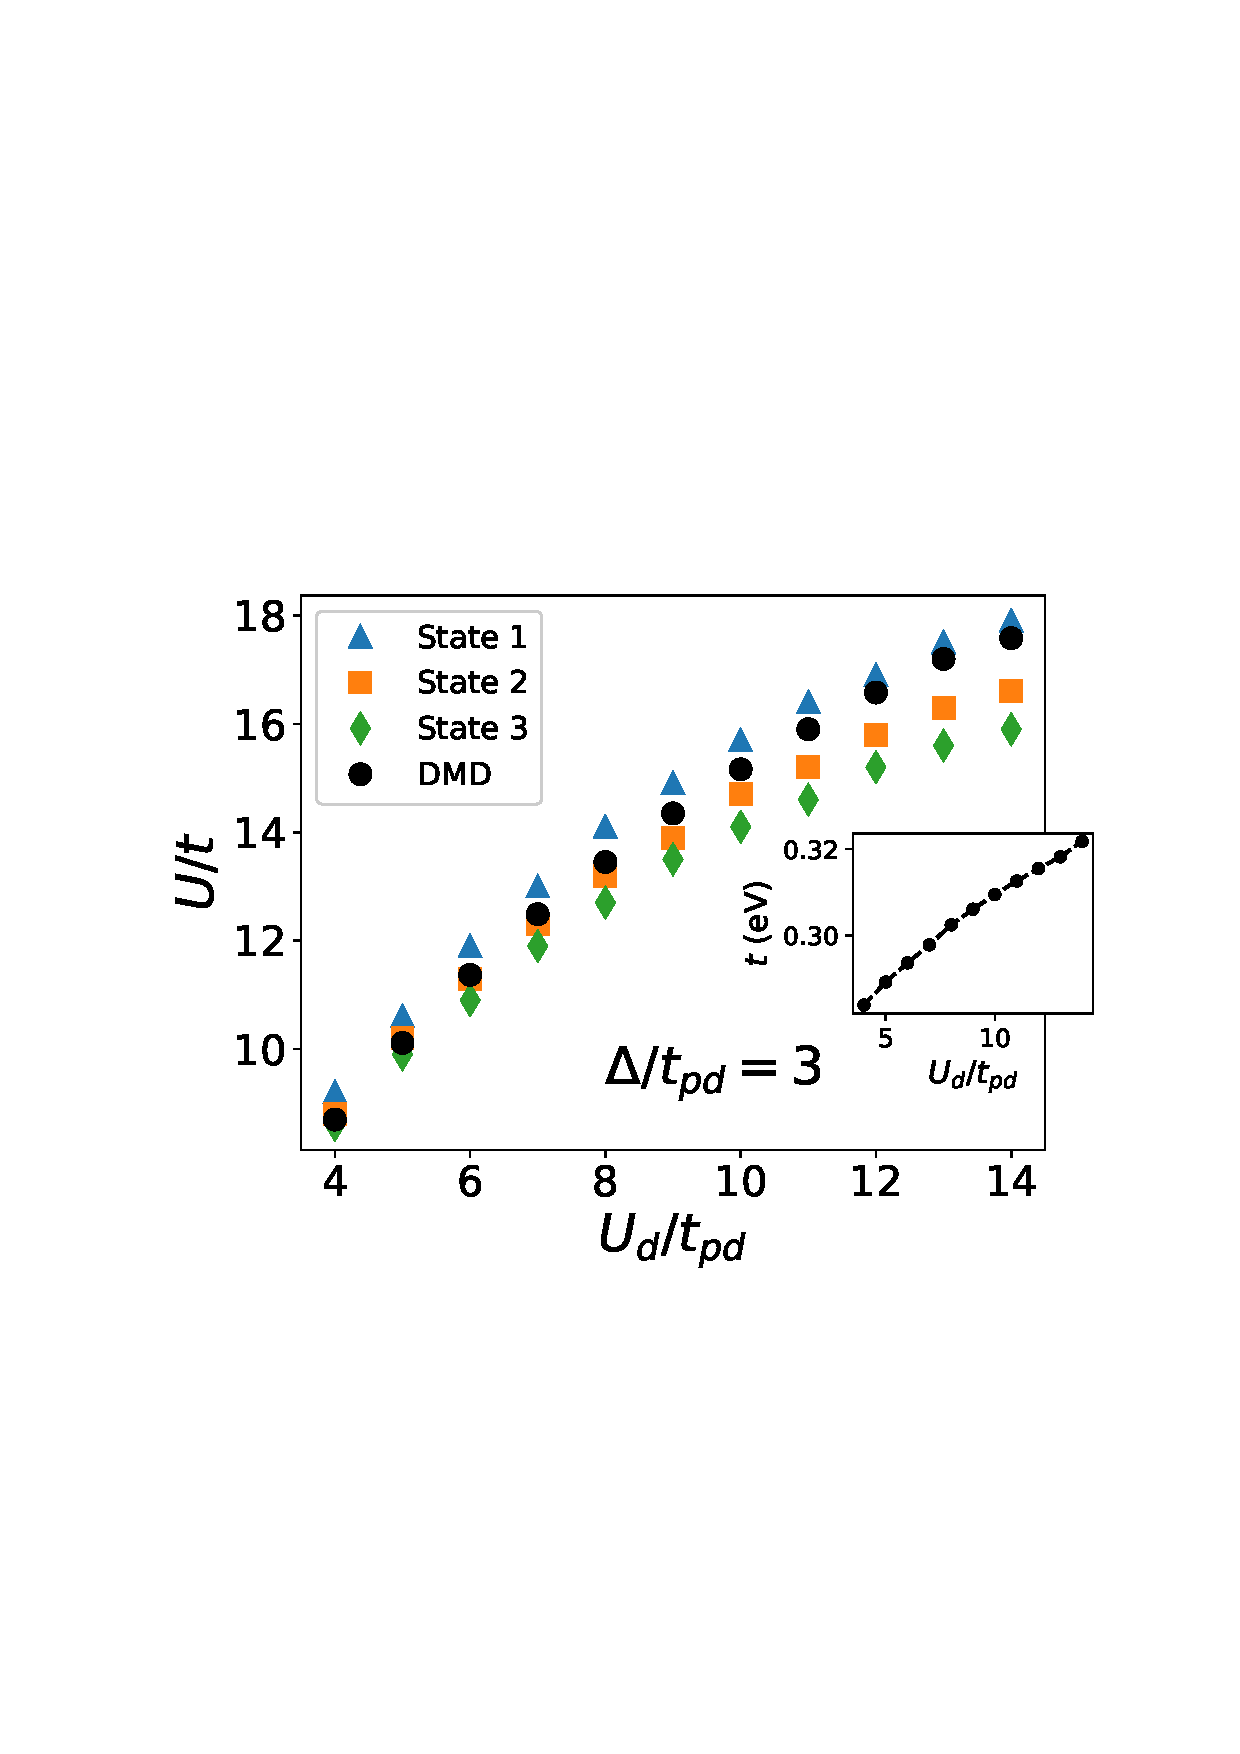
\includegraphics[width=0.48\linewidth]{./Figures/U_and_hopping_combined_vs_Ud_ep_3.pdf}
\includegraphics[width=0.50\linewidth]{./Figures/U_and_hopping_combined_vs_Ud_ep_5.pdf}
\caption{Downfolded values of the effective 1-band Hubbard $U/t$ and $t$ (inset) 
vs $U_d/t_{pd}$ for two representative values of $\Delta/t_{pd}$}
\label{fig:hamfitUdvary} 
\end{figure}	
 
We now explore the validity of the 1-band description by monitoring 
the trends associated with the downfolded parameters as a function of varying $\Delta/t_{pd}$ and 
$U_d/t_{pd}$. Fig.~\ref{fig:hamfitepdvary} shows our results for the optimal 
transformation parameters ($\alpha$'s), $t$ and $U/t$ as a function of $\Delta/t_{pd}$
keeping $U_d/t_{pd}=8$ fixed. Prominently, 
$\alpha_1$, which is the parameter that mixes the copper and its nearest neighbor oxygen orbitals, 
\textit{decreases} as $\Delta/t_{pd}$ is increased. 
This is physically reasonable since an increasing difference in the single particle energies of the copper and oxygen orbitals 
means the increased unfavorableness of holes to occupy the latter. 
Correspondingly the effective hopping in the 1-band model reduces and the effective $U/t$ increases. 

Next, in Fig.~\ref{fig:hamfitUdvary} analogous results are presented by fixing $\Delta/t_{pd}$ 
to two representative values, and varying $U_d/t_{pd}$. In both cases, $U/t$ increases 
dramatically with $U_d/t_{pd}$, but $t$ changes only marginally; the hybridization parameters also follow this trend. 
Also, the different estimates of $U/t$ are closer to each other for the case of larger $\Delta$ 
indicating the increased effectiveness of the 1-band model. 

One important check for the downfolded model is its ability to reproduce the low energy spectrum of 
the full model. Fig.~\ref{fig:energyfit} shows the comparison of the lowest six eigenstates of the 
1-band and 3-band models. These six states correspond to 4C2 states of the effective spin model 
in its $S_z=0$ sector, all of which correspond to \textit{d like} spin excitations. 
The eigenstates above this manifold involve \textit{p-like} excitations, an aspect the 1-band model is not designed to capture. 
In all cases, the fit is reasonably good from an energetic viewpoint; the best fits seen at larger 
$U_d$ and larger $\Delta$ consistent with our expectations from the previous plots. Despite this good agreement, 
we caution that the reduced sensitivity of the energy to small RDM elements means 
that the Hubbard parameters (from the standard protocol or eigenstate matching) 
can be strongly dependent on the energy window of interest, a point we highlight shortly. 
%We re-emphasize that once the density matrices were transformed %only one parameter ($t$) was fit to match five energy gaps between the two models; this indicates %it is thus an indicator of the success of the downfolding (rather than a result of overfitting). 
\begin{figure}[]
\centering
\includegraphics[width=0.325\linewidth]{./Figures/Gap_1_band_3_band_ep_3_number_5.pdf}
\includegraphics[width=0.325\linewidth]{./Figures/Gap_1_band_3_band_ep_3_number_9.pdf}
\includegraphics[width=0.325\linewidth]{./Figures/Gap_1_band_3_band_ep_3_number_2.pdf}
\includegraphics[width=0.325\linewidth]{./Figures/Gap_1_band_3_band_ep_5_number_5.pdf}
\includegraphics[width=0.325\linewidth]{./Figures/Gap_1_band_3_band_ep_5_number_9.pdf}
\includegraphics[width=0.325\linewidth]{./Figures/Gap_1_band_3_band_ep_5_number_2.pdf}
\caption{Comparison for energy gaps between the 3-band and 1-band Hubbard models 
using the optimized values of $U/t$ and $t$, for different $U_{d}/t_{pd}$ for $\Delta/t_{pd}=3$ (top row) 
and $\Delta/t_{pd}=5$ (bottom row)}
\label{fig:energyfit} 
\end{figure}	

We motivated the need for downfolding by suggesting that one of its primary objectives 
is to reduce the size of the effective Hilbert space; the downfolded Hamiltonian enables 
simulations of a bigger unit cell. To show that this actually works well in practice for the 3-band case, 
we consider the $2\sqrt{2} \times 2 \sqrt{2}$ square unit cell, comprising of 8 copper and 16 oxygen orbitals. 
For the six test cases presented in Fig.~\ref{fig:energyfit}, we performed an exact diagonalization 
(or full configuration interaction) calculation at half filling, the Hilbert space comprises of 112911876 basis states. 
Roughly 200 Lanczos iterations were carried out, enabling convergence of the lowest four energies. 
We compared the lowest gaps with the corresponding calculation on the single 
band model with the same square geometry (Hilbert space size of only 4900) using the downfolded 
parameters obtained from the smaller $2 \times 2$ cell. Our results are summarized in Table xx

\begin{table}[ht]
\centering
\begin{tabular}{c||c|c||c|c||c|c|}
\hline
Case                             & $E_1-E_0$ & $E_1-E_0$ & $E_2-E_0$ & $E_2-E_0$ & $E_3-E_0$ & $E_3-E_0$ \\
\hline
$\Delta/t_{pd}$=3,$U_d/t_{pd}=4$ &           &           &           &           &           &        \\ 
$\Delta/t_{pd}$=3,$U_d/t_{pd}=8$ &           &           &           &           &           &        \\
$\Delta/t_{pd}$=3,$U_d/t_{pd}=12$ &           &           &           &           &           &       \\
\hline
\hline
$\Delta/t_{pd}$=5,$U_d/t_{pd}=4$ &           &           &           &           &           &        \\
$\Delta/t_{pd}$=5,$U_d/t_{pd}=8$ &           &           &           &           &           &        \\
$\Delta/t_{pd}$=5,$U_d/t_{pd}=12$ &           &           &           &           &           &       \\
\hline
\hline
\end{tabular}
\label{tab:predictivity}
\end{table} 

\HJC{Once the predicitivity objective is achieved for the lowest eigenstates, discuss the 6 test cases with N-AIDMD. 
This gets the average parameters that best describes the energy window, not only the extrema}


